\documentclass[dvips, 12pt]{article}

% Any percent sign marks a comment to the end of the line

% Every latex document starts with a documentclass declaration like this
% The option dvips allows for graphics, 12pt is the font size, and article
%   is the style


\newcommand*{\TitleFont}{%
		\usefont{\encodingdefault}{\rmdefault}{b}{n}%
		\fontsize{16}{20}%
		\selectfont}

\newcommand{\HRule}{\rule{\linewidth}{0.5mm}}



\usepackage{graphicx}
\usepackage{url}
\usepackage{harmony}
\usepackage{musixtex}

% These are additional packages for "pdflatex", graphics, and to include
% hyperlinks inside a document.

\setlength{\oddsidemargin}{0.25in}
\setlength{\textwidth}{6.5in}
\setlength{\topmargin}{0in}
\setlength{\textheight}{8.5in}

% These force using more of the margins that is the default style


% Everything after this becomes content
% Replace the text between curly brackets with your own

\title{{\Huge \bfseries SMURF} \\ \Large \it Serial MUsic Represented as Functions \vspace{0.6cm}}

\author{\normalsize Richard Townsend, Lianne Lairmore, Lindsay Neubauer, Van Bui, Kuangya Zhai
	\\ \small \{rtownsend, lairmore, neubauer, vbui, kyzhai\}@cs.columbia.edu \vspace{0.6cm}}

\date{\today \vspace{2cm}}

% You can leave out "date" and it will be added automatically for today
% You can change the "\today" date to any text you like

\begin{document}
\maketitle


% This command causes the title to be created in the document

\section{Introduction}

% An article style is separated into sections and subsections with 
%   markup such as this.  Use \section*{Principles} for unnumbered sections.

Each working group should prepare a brief proposal describing what they want 
to do.  Please make sure that everyone participates in the discussions and
reviews the document.  The usual way to do this is to have a principle author,
but to pass it around so that everyone can comment and add or edit.  Prepare the
document using \LaTeX\/ because it is good practice and will help you learn the
basics.  However, note that Google Docs (a.k.a. Google Drive) also allows
\LaTeX\/ math symbols and is a reasonable alternative except for submissions
to journals for professional use.  There is help for \LaTeX\/ on the
class website.

Write a brief introduction in which you  outline the scope of your proposed
work. Use this space to explain why you are interested in this topic and what
you hope to learn. Connect your interest with what is currently known, and
include at least two references to related articles in the astronomical
literature.  You can use ADS  \url{http://adswww.harvard.edu/} and other links
on the class website \url{http://prancer.physics.louisville.edu/classes/308/} 
to help you find out more. An example citation is this paper
\cite{gonzalez2012}.

One to two pages should suffice for this part, but use more if you want.  
Include figures or images if needed.  Figure~\ref{m42} is an example of  how to
do it in \LaTeX.


\begin{figure}
\begin{center}
\resizebox{6in}{!}{\includegraphics*{figures/hello}}
\end{center}

\caption{The first picture\label{m42}}
\end{figure}


\begin{figure} % use float package if you want it here
  \centering
  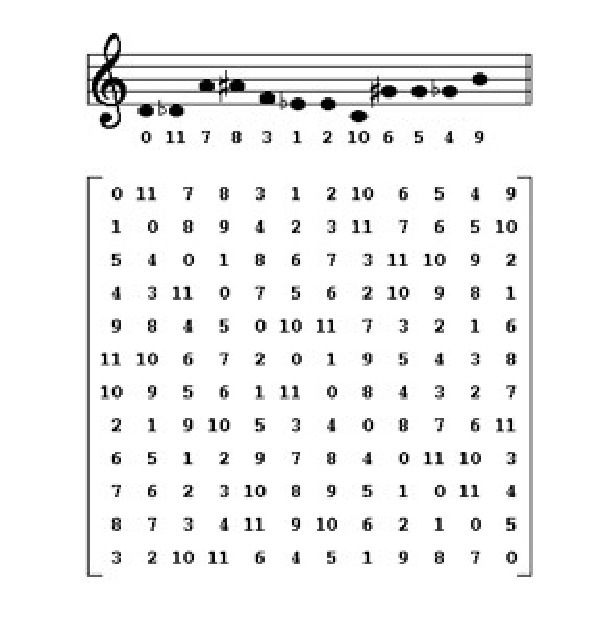
\includegraphics[width=10cm]{figures/Matrix}
  \caption{The second picture}
  \label{fig:xfig1}
\end{figure}



\section{Motivation}

Our group has decided to create a language that will assist a composer in creating music 
using the twelve tone method described above. We plan on making this language 
functional and compile into C. The compilation process will create a C program 
that will use openGL to create an image representing the music created. 

Twelve tone serialism is a mathematically intensive method of creating music which 
involves mapping notes to numbers. It is very natural to work with twelve tone rows 
using a programming language since the method just treats notes like numbers that 
can be added and subtracted from. We plan on our language making twelve tone compilation 
easier using data types and functions specifically for the purpose of creating music in 
this way. By simplifying the method of inverting and transposing rows composers can focus 
more on how to exploit new ways to make music in this fashion and worry less about 
creating matrices. 

We chose to implement our language as a functional language because of the clear and 
succinct programs that functional languages produce. It also makes sense for our language 
to be functional because functional languages also are well known for their ability to 
work on lists and most arithmetic done in twelve tone serialism is done on rows or 
columns. As a group we are also very interested on how a functional language compiler 
works. 

Instead of compiling our language into byte code which can be interpreted and play the 
notes we thought it would be more interesting to create a language that could be compiled 
into a score. Scores are made up of just lines and dots and would be easy to create in 
a graphics library like openGL. We decided to compile our language into C since it was a 
significantly less abstract language which had access to openGL library calls. One benefit 
of compiling into C and not a language to be interpreted as music is that programs in our 
language could be created that do not actually output any music but instead create 
functions that could be used in other programs to do the same transformation of rows. 
That way our language is not just limited to functions defined in our libraries or 
what is in the current file. 

Overall we hope to use the simplicity of a functional language to help composers write 
complex, new, and interesting music based on twelve tone serialism. These new compositions 
would then be able to be printed and handed to musicians to play. This simplifies the 
composers task of converting music in computer format to one which musicians will be 
able to read easily. 

\section{Syntax}

SMURF is a functional programming language loosely modeled off of Haskell. It has immutable memory, no global variables and no I/O.

\subsection{Types}

\subsubsection{Standard Types}
\begin{itemize}
\item Integer: int
\item Boolean: bool
\item Tuples: elements can have different types
\item Lists: elements must have same type
\end{itemize}

\subsubsection{Note (pc: int, beat: int, register: int)}
\begin{itemize}
\item pc (pitch class): represented by integers 0-11
\item beat: represented by powers of 2 up to 32 (assuming \Takt{4}{4} time)
\item register: represented by integers -2 to 2
  \begin{itemize}
  \item \begin{music}  \trebleclef  \end{music}  Treble Clef: notes middle C and higher represented by 0-2  
  \item \begin{music} \bassclef  \end{music}  Bass Clef: notes lower than middle C represented by negative numbers
  \end{itemize}
\end{itemize}

\subsubsection{Chord ([Note])}
\begin{itemize}
\item Type checks that all notes have same beat count
\end{itemize}

\subsubsection{Figure ([Chord])}

\subsubsection{Functions}
A function is a type whose value can be defined with an expression
\begin{itemize}
\item Function declarations must declare type (can declare general type)
\item Function declarations must be on own line
\item No explicit return
\item Pattern matching, guards, and if-then-else clauses used
  \begin{itemize}
  \item Each pattern matching pattern must be on own line
  \item Guards and if-then-else clauses do not have newline restrictions
  \end{itemize}
\end{itemize}

\begin{table} [h]
	\centering
    \begin{tabular}{ll}
    \hline\hline
    Operators & \\
    \hline\hline
       \textbackslash n & End of line: Terminates phrases \\ \hline
      + & Integer arithmetic: plus  \\ \hline
      - & Integer arithmetic: minus  \\ \hline 
      \% & Integer arithmetic: modulus, ignores negatives  \\ \hline
      \textless  & Comparison \\ \hline
      \textgreater  & Comparison \\ \hline
      \textless=  & Comparison \\ \hline
      \textgreater= & Comparison \\ \hline
       == & Structural comparison  \\ \hline
       not & Boolean operator \\ \hline
       \&\& & Boolean operator \\ \hline
       \textbar\textbar & Boolean operator \\ \hline
      ++ & Concatenation: concat \\ \hline
      : & Construction: cons \\ \hline
      /* */ & Multiline comments, nesting allowed \\ \hline
      // & Single-line comment \\ \hline
    \end{tabular}
\end{table}

\begin{table} [h]
	\centering
    \begin{tabular}{ll}
    \hline\hline
    Keywords & \\ 
    \hline\hline
      let & Specify values and functions  \\ \hline
      \textendash\textgreater & Specify arguments and return type of functions  \\ \hline
      :: & Specify types \\ \hline
      if, then, else & Specify conditional expression, else compulsory  \\ \hline
      \textbar & Specify boolean expression, used with guards\\ \hline
    \end{tabular}
\end{table}





 


\section{SMURF Examples}

In this section, we provide two examples that use a variety of language features in SMURF.

\subsection{Simple Example}
The simple SMURF program shown in Figure~\ref{fig:example1} first defines the pitch classes for the prime row in line 1. Using the prime row as a base, the program creates a score with a single measure using the notes generated by transposing the prime row by three semitones (line 2), inverting the resulting transposed row (line 3), and then reversing the inverted row from the prior step (line 4). Lines 2-4 use the \emph{trans, inver, and rev} library routines to apply transposition, inversion, and reversal to a list, respectively. Line 5 invokes a library routine called \emph{rowToNotes} that converts each pitch class in a tone row to a list of notes given beat and register value mappings for each pitch class in the tone row. For simplicity, all the notes in this example are quarter notes (4) in register 0. Line 6 defines a measure using the first two notes in the list of notes returned in line 5; the second half of the measure consist of two rest quarter notes in register 0.  Line 7 uses the keyword \textbf{genScore} along with the measure defined in the prior line as an argument. The compiler translates the keyword \textbf{genScore} down to C+OpenGL code to create a score sheet based on the given list of measures.     

\begin{figure}
  \centering
  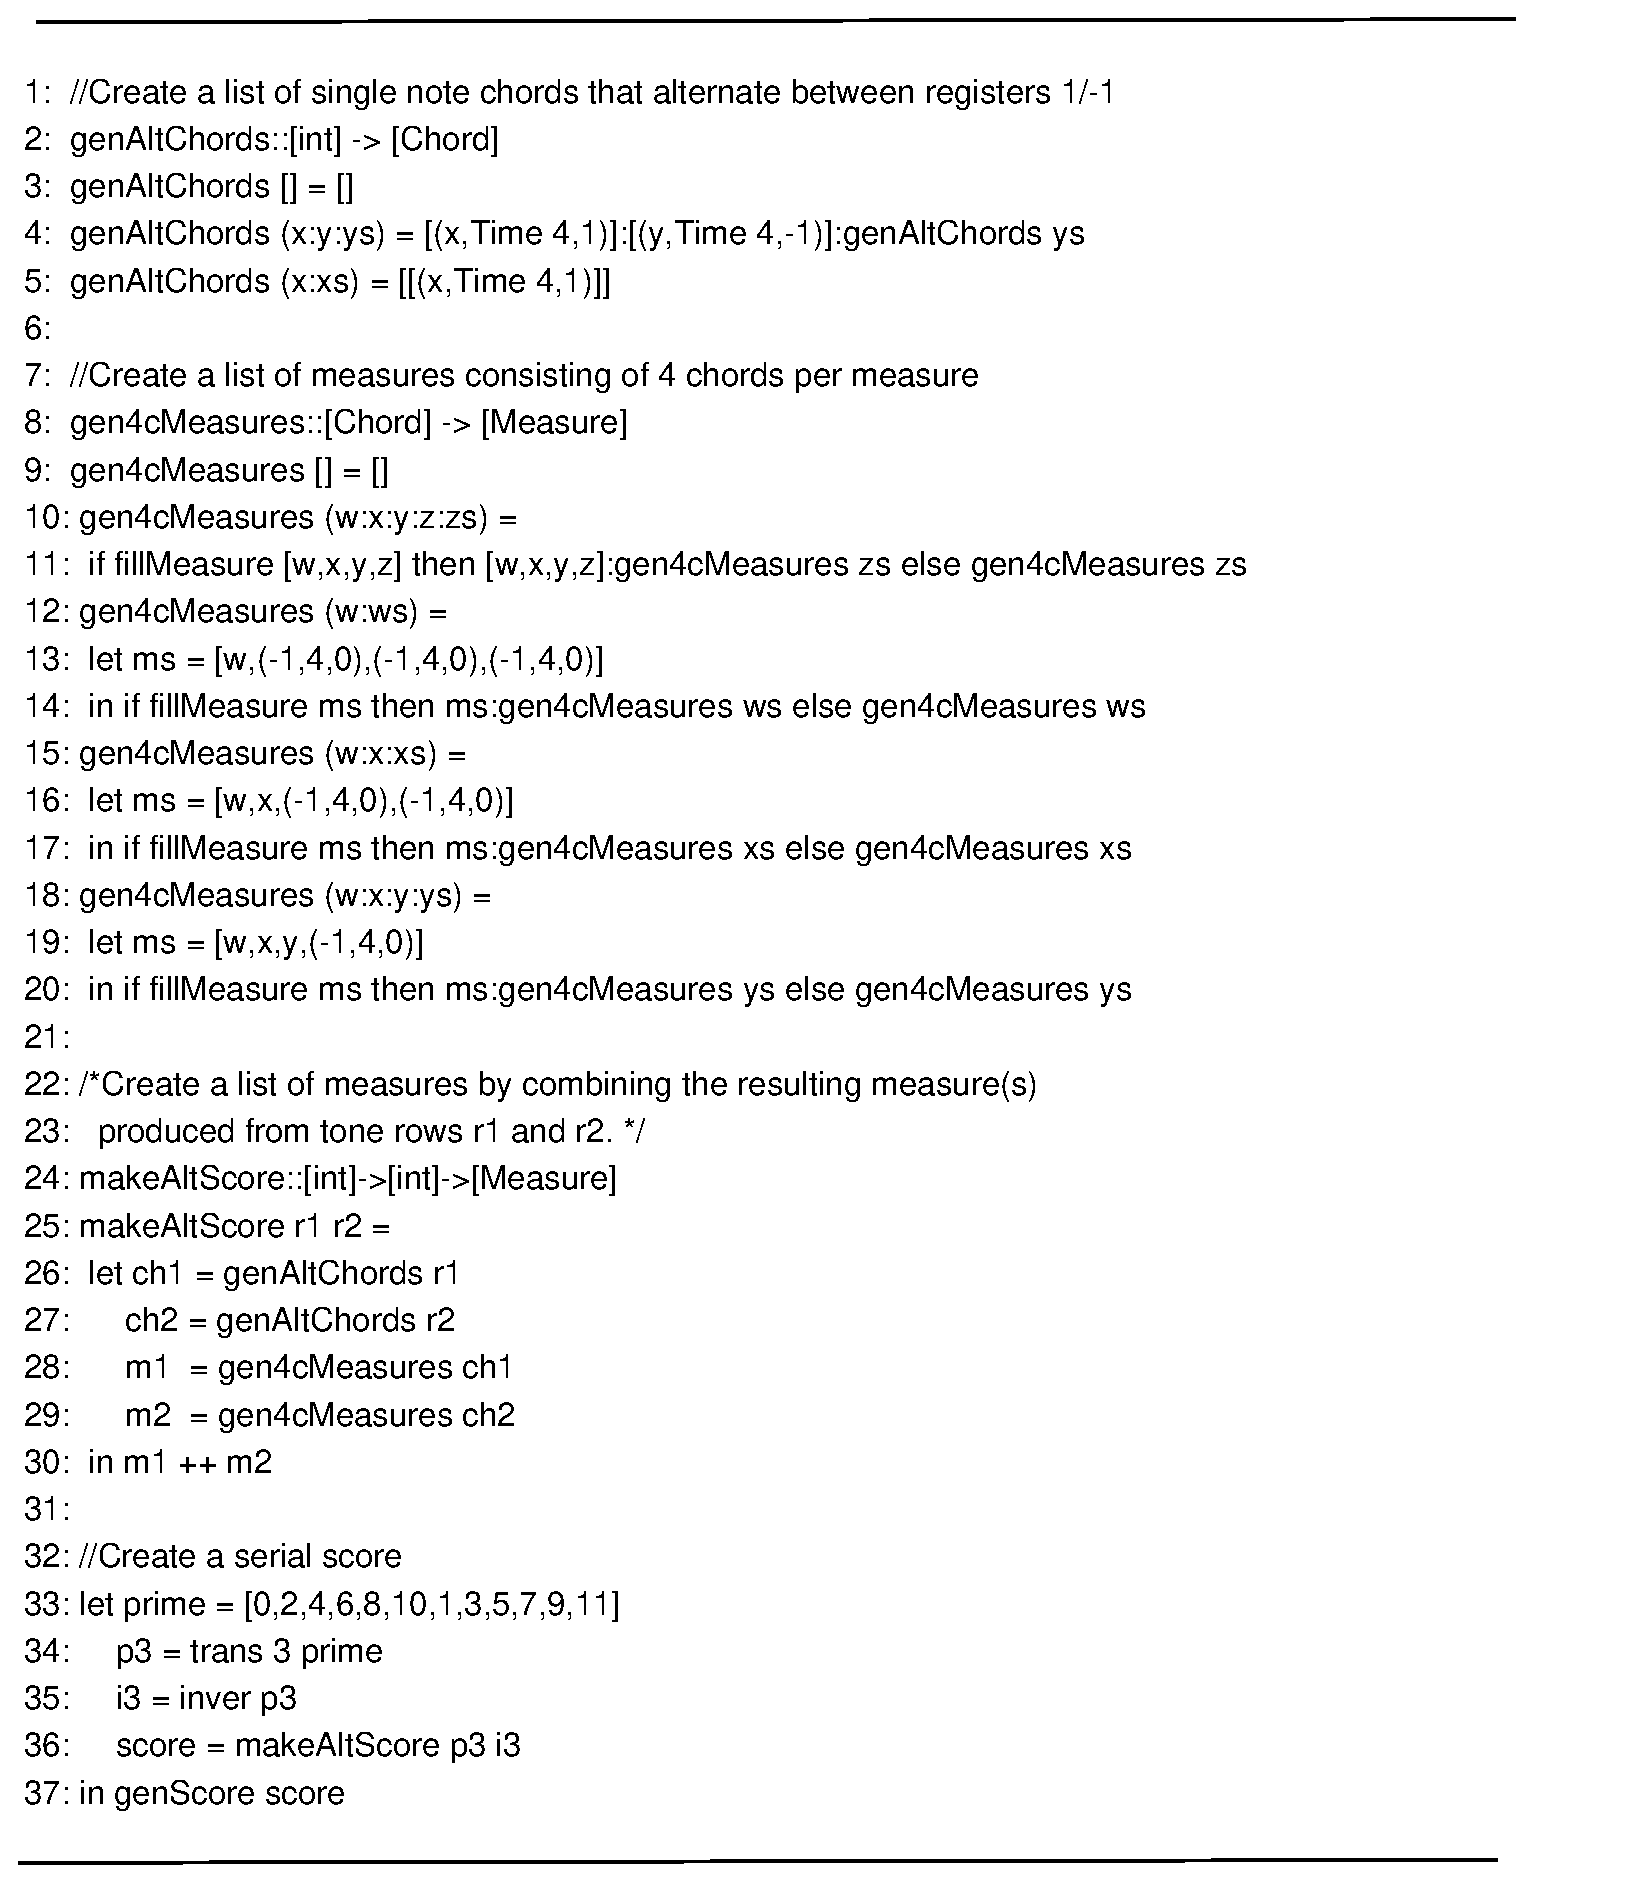
\includegraphics[width=\textwidth]{figures/example1}
  \caption{Simple SMURF example code. The code uses the trans, inver, and rev library routines to generate a tone row that is then used to create notes, a measure, and then finally a score.}
  \label{fig:example1}
\end{figure}

\subsection{Second Example}

The example code presented in Figure~\ref{fig:example2} shows how to define functions, use keywords, use types, and apply operators in SMURF. 

\begin{figure}
  \centering
  \includegraphics[width=\textwidth]{figures/example2}
  \caption{This SMURF code takes in the p3 and i3 tone rows from Figure~\ref{fig:example1} and generates a score consisting of notes that alternate between the -1 and 1 registers.}
  \label{fig:example2}
\end{figure}

% comment out
\iffalse
\small
\begin{verbatim}
1: prime = [0,2,4,6,8,10,1,3,5,7,9,11]
2: p3    = trans 3 prime
3: i3    = inver p3
4: ri3   = rev i3
5: firstNotes = rowToNotes ri3 [4,4,4,4,4,4,4,4,4,4,4,4] [0,0,0,0,0,0,0,0,0,0,0,0]
6: firstMeasure = head firstNotes:(head (tail firstNotes)):(-1,4,0):(-1,4,0):[]
7: genScore [firstMeasure]
\end{verbatim}

\small
\begin{verbatim}
1: //create a list of chords that alternate between registers 1/-1
2: genAltChords::(int a,chord b)->[a]->[b]
3: genAltChords [] = []
4: genAltChords (x:y:ys) = [(x,4,1)]:[(y,4,-1)]++genAltChords ys
5: 
6: //create a list of measures consisting of 4 chords in each measure
7: gen4cMeasures::(chord a, measure b)->[a]->[b]
8: gen4cMeasures [] = []
9: gen4cMeasures (w:x:y:z:zs) = [w:x:y:z] ++ genMeasures zs
10:
11: /*create a score based on combining the measures produced
12:   from applying two tone rows to genChords */
13: makeAltScore::(int a, score c) -> [a]->[a]->[c]
14: makeAltScore r1 r2 = 
15:    let ch1 = genAltChords r1
16:        ch2 = genAltChords r2
17:        m1  = gen4cMeasures ch1
18:        m2  = gen4cMeasures ch2
19:    in m1 ++ m2 
20:
21: let score = makeAltScore p3 i3 
22: in genScore [score]
\end{verbatim}
\fi



% citations begin here
\bibliographystyle{ieeetr}
\bibliography{ref/refs}


\end{document}
